\subsection{Titulos}
   \hypertarget{subsec:titulos}
   Se muestran en la figura \ref{fig:titulo} los títulos y certificados relacionados a la carrera de grado.
   \begin{figure}
      \begin{center}
         \begin{subfigure}[b]{0.45\textwidth}
            
\includegraphics[width=\textwidth, frame]{portfolio/titulo_itba.jpg}
            \caption{Título de Ingeniero Electrónico con especialidad en Telecomunicaciones del ITBA.}
            \label{fig:titulo_itba}
         \end{subfigure}%
         \hfill
         \begin{subfigure}[b]{0.45\textwidth}
            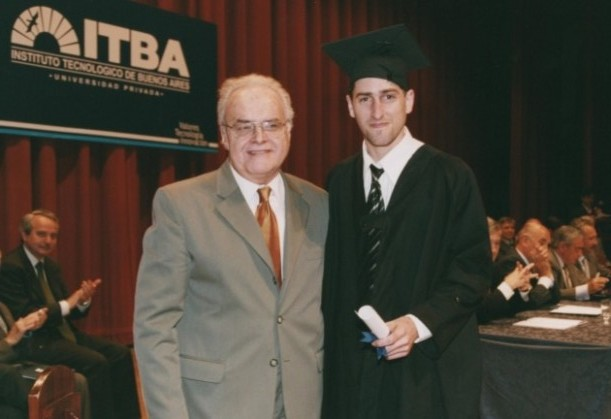
\includegraphics[width=\textwidth, frame]{portfolio/foto_entrega_titulo.jpg}
            \caption{Foto de entrega de título junto con mi profesor y referente, el Ing. Informático .}
            \label{fig:foto_titulo}
         \end{subfigure} %
         \begin{subfigure}[b]{0.40\textwidth}
            \begin{center}
               
\includegraphics[width=0.6\textwidth, frame]{portfolio/medalla_i+d_1.jpg}
               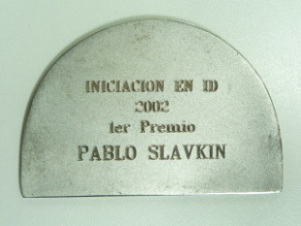
\includegraphics[width=0.6\textwidth, frame]{portfolio/medalla_i+d_2.jpg}
               \caption{Medalla al primer puesto en I+D, iniciación en investigación y desarrollo, del ITBA}
               \label{fig:medalla_i+d}
            \end{center}
         \end{subfigure}%
         \hfill
         \begin{subfigure}[b]{0.55\textwidth}
            
\includegraphics[width=\textwidth, frame]{portfolio/robot.jpg}
            \caption{Certificado de participación en Batletek, competencia de lucha de robots en el ITBA, en donde se obtuvo el tercer puesto.}
            \label{fig:foto_robot}
         \end{subfigure}%
      \caption{Títulos y certificados obtenidos durante la carrera de grado en el ITBA.}
      \label{fig:titulo}
      \end{center}
   \end{figure}

   \begin{figure}
      \begin{center}
      \ContinuedFloat
         \begin{subfigure}[b]{0.45\textwidth}
            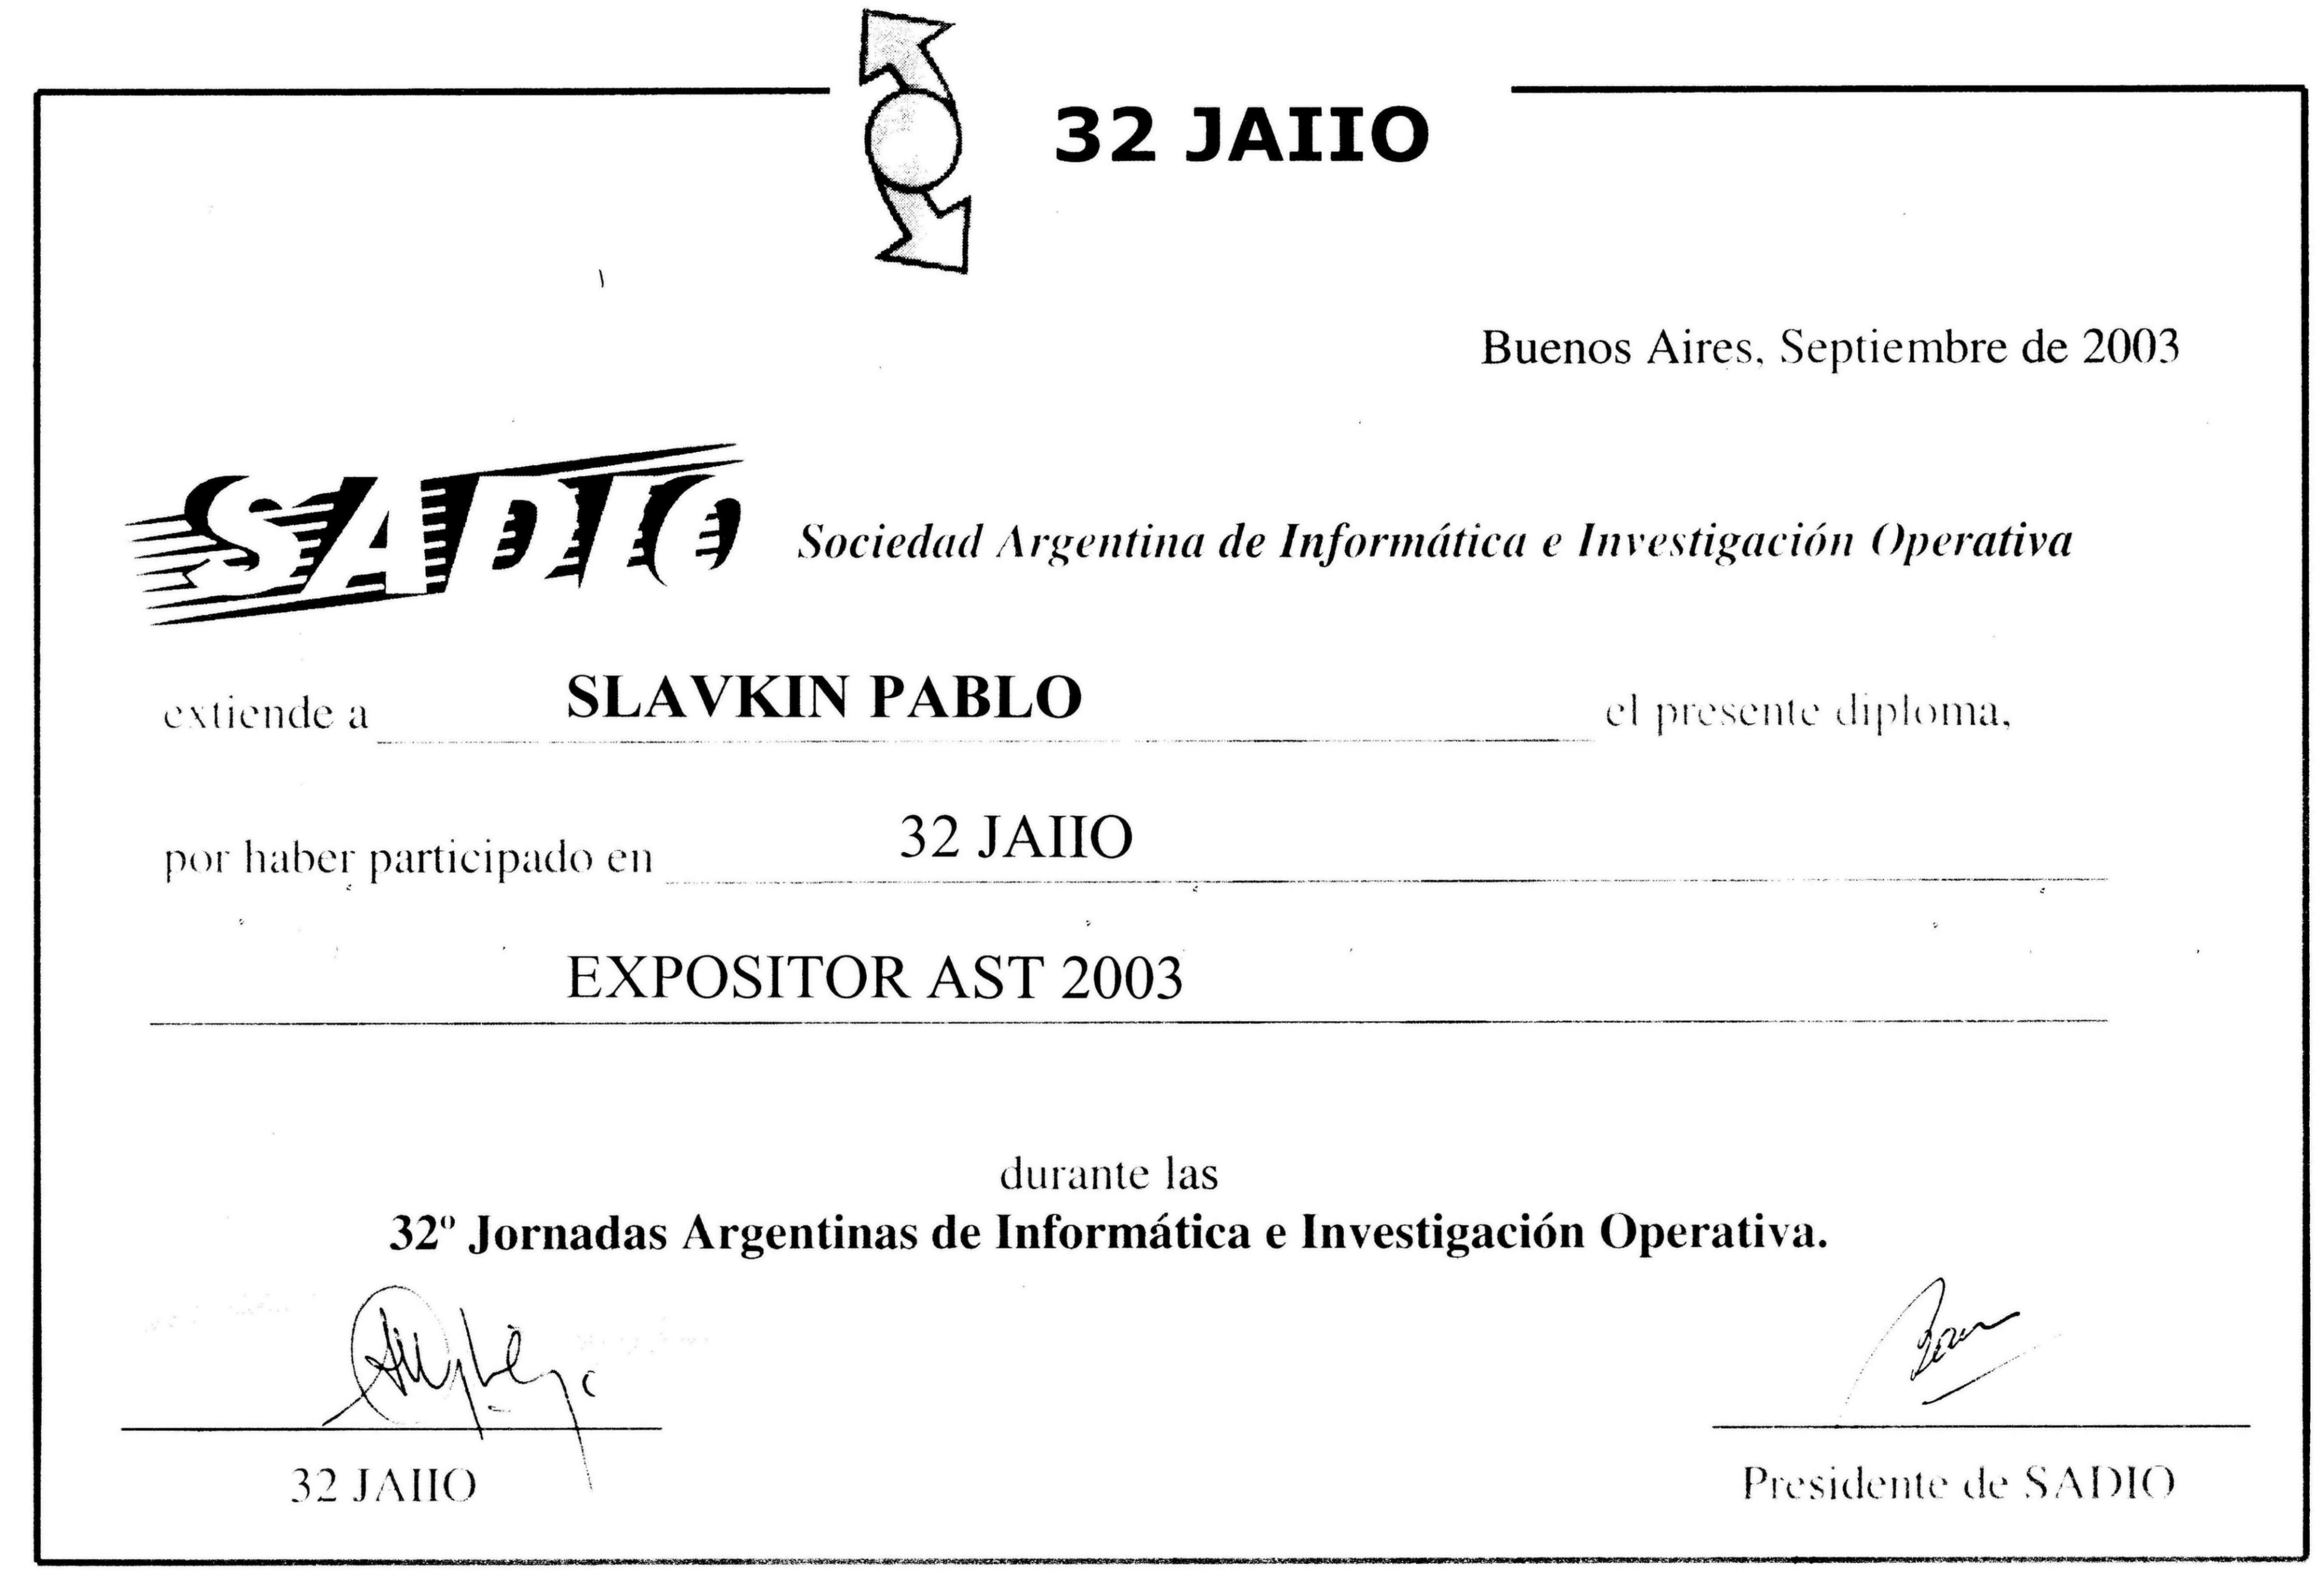
\includegraphics[width=\textwidth, frame]{portfolio/sadio.jpg}
            \caption{JAIIO, 32\textsuperscript{o} Jornadas Argentinas de Informática e Investigación Aplicada. Se presento el trabajo \emph{Design and Simulation of a pipeline-structured Floating Point Unit for high performance general purpose processors.} \href{https://drive.google.com/open?id=15NkqA_rWbaObx1uiqe7ruBg9lWpIh5q7}{ver trabajo}}
            \label{fig:jaiio}
         \end{subfigure}%
         \hfill
         \begin{subfigure}[b]{0.45\textwidth}
            
\includegraphics[width=\textwidth, frame]{portfolio/cacic.jpg}
            \caption{CACIC, IX Congreso Argentino de Ciencias de la Computación en donde se presento el trabajo \emph{Selection of the Optimum Stage Number in Pipelined Floating-Point Units} \href{https://drive.google.com/open?id=11z5qRrJ01Is6dx5NMHAOoXl3D0r2o8OY}{ver trabajo}}
            \label{fig:cacic}
         \end{subfigure}%
      \end{center}
      \caption{Títulos y certificados obtenidos durante la carrera de grado en el ITBA.}
      \label{fig:titulo}
   \end{figure}
